% Mitigating User Interface Latency Caused by Event Accumulation in an
% Online Video Editor Built on a Client-Server Architecture
% Copyright (C) 2012  Michael Chang
% based on
% uw-wkrpt-se.tex - An example work report that uses uw-wkrpt.cls
% Copyright (C) 2002,2003  Simon Law
% 
% This program is free software; you can redistribute it and/or modify
% it under the terms of the GNU General Public License as published by
% the Free Software Foundation; either version 2 of the License, or
% (at your option) any later version.
% 
% This program is distributed in the hope that it will be useful,
% but WITHOUT ANY WARRANTY; without even the implied warranty of
% MERCHANTABILITY or FITNESS FOR A PARTICULAR PURPOSE.  See the
% GNU General Public License for more details.
% 
% You should have received a copy of the GNU General Public License
% along with this program; if not, write to the Free Software
% Foundation, Inc., 59 Temple Place, Suite 330, Boston, MA  02111-1307  USA
%
%%%%%%%%%%%%%%%%%%%%%%%%%%%%%%%%%%%%%%%%%%%%%%%%%%%%%%%%%%%%%%%%%%%%%
%
% We begin by calling the workreport class which includes all the
% definitions for the macros we will use.
\documentclass[se,resubmit]{uw-wkrpt}

% LaTeX preamble: load some packages to add functionality
\usepackage{graphicx} % Include graphic importing

\usepackage[T1]{fontenc} % Better fonts
\usepackage{ae,aecompl}

\usepackage{indentfirst} % Indent first paragraph of each section

\usepackage[titletoc,title]{appendix} % Prefix appendix letters with `Appendix'

% For mathematical symbols in our pseudocode
\usepackage{amsmath}

% Use the algorithmicx package for pseudocode
\usepackage{algorithm}
\usepackage{algpseudocode}

% Use biblatex for references
\usepackage[style=ieee,sorting=none,dateabbrev=false,backend=biber]{biblatex}
\addbibresource{report.bib} % Specify the bibliography file

\usepackage{listings}

% This needs to be the last package loaded
\usepackage[pdftex]{hyperref} % Generate PDF links and bookmarks.
\hypersetup{
  bookmarks=true,
  bookmarksnumbered=true
}

% Now we will begin writing the document.
\begin{document}

%%%%%%%%%%%%%%%%%%%%%%%%%%%%%%%%%%%%%%%%%%%%%%%%%%%%%%%%%%%%%%%%%%%%%
%% IMPORTANT INFORMATION
%%%%%%%%%%%%%%%%%%%%%%%%%%%%%%%%%%%%%%%%%%%%%%%%%%%%%%%%%%%%%%%%%%%%%

%% First we, should create a title page.  This is done below:
% Fill in the title of your report.
\title{ Mitigating User Interface Latency Caused by Event Accumulation in an
Online Video Editor Built on a Client-Server Architecture }

% Fill in your name.
\author{Michael Chang}

% Fill in your student ID number.
\uwid{20332377}

% Fill in the name of the PNG file with your signature, or leave unchanged.
\signature{signature}

% Fill in your home address.
\address{30 Doncrest Rd.\\*
         Richmond Hill, ON\ \ L4B 1A2}

% Fill in your employer's name.
\employer{Google Inc.}

% Fill in your employer's city and province.
\employeraddress{Mountain View, CA}

% Fill in your school's name.
\school{University of Waterloo}

% Fill in your faculty name.
\faculty{Software Engineering}

% Fill in your student user ID
\userid{m9chang}

% Fill in your e-mail address.
\email{m9chang@uwaterloo.ca}

% Fill in your term.
\term{3A}

% Fill in your program.
\program{Software Engineering}

% Fill in the department chair's name.
\chair{Dr.\ A.\ Morton}

% Fill in the department chair's mailing address.
\chairaddress{Software Engineering\\*
              University of Waterloo\\*
	      Waterloo, ON\ \ N2L 3G1}

% If you are writing an "SE-confidential" report, uncomment the next line.
%\confidential{SE-confidential}

% If you want to specify the date, fill it in here.  If you comment out
% this line, today's date will be substituted.
\date{December 15, 2012}

% Now, we ask LaTeX to generate the title.
\maketitle

%%%%%%%%%%%%%%%%%%%%%%%%%%%%%%%%%%%%%%%%%%%%%%%%%%%%%%%%%%%%%%%%%%%%%
%% FRONT MATTER
%%%%%%%%%%%%%%%%%%%%%%%%%%%%%%%%%%%%%%%%%%%%%%%%%%%%%%%%%%%%%%%%%%%%%
%% \frontmatter will make the \section commands ignore their numbering,
%% it will also use roman page numbers.
\frontmatter

% After this, we must create a letter of submission.
\begin{letter}
I have completed my fourth work term, following my \theterm{} term. Please find
enclosed my third work term report entitled: ``\thetitle'' for YouTube, LLC, a
subsidiary of \theemployer.  My manager was B. Glickstein, and our team was
primarily involved with building tools for video creators and content curators.

This report focuses on the handling of input events in the video
enhancement tool on YouTube. This problem is similar to one that I
encountered on my work term, but has been modified to protect proprietary
design decisions.

I wish to thank B. Glickstein and R. Doshi for their advice on the
technical content of this report. I also wish to thank C. Kleynhans and M.
Yee for their advice on choosing a word processing environment to write
this report, and W. Chang for proofreading this report. Finally, I
wish to thank A. Mortezaei for providing feedback on the initial
submission of this report.

% Note that I do not need to type out the boilerplate confirmation,
% nor do I need to write a signature block.  This is generated for me.
% We are now finished with the letter.
\end{letter}

% We continue with required sections, such as the Executive Summary.
\section{Executive Summary}
AudioSwap is one of the video enhancement features available to video
creators on YouTube. It allows video creators to select a song from a
library of over 100,000 songs that YouTube has licensed. The initial
implemention of AudioSwap only allowed users to place the audio at the
beginning of their video, and to use the song in its entirety. One of the
major accomplishments of my work term was to implement user interface
changes which allow video creators to position and trim tracks they've
placed over their videos using AudioSwap.

This document describes issues which arose when these changes were first
publicly deployed. It also describes some ways those issues could be
mitigated, and uses the multi-criteria decision making methdology to rank
these mitigation strategies. Finally, it discusses these issues in the
context of the material in CS 349 - User Interfaces, which is a core
course in the Software Engineering curriculum, and presents some general
considerations for adapting the lessons learned from the issues presented
to future software projects.

% Next, we need to make a Table of Contents, List of Figures and 
% List of Tables.  You will most likely need to run LaTeX twice to
% get these correct.  The first pass for LaTeX to figure out the
% labels, and the second pass to put in the right references.
\tableofcontents
\listoffigures
\listoftables

%%%%%%%%%%%%%%%%%%%%%%%%%%%%%%%%%%%%%%%%%%%%%%%%%%%%%%%%%%%%%%%%%%%%%
%% REPORT BODY
%%%%%%%%%%%%%%%%%%%%%%%%%%%%%%%%%%%%%%%%%%%%%%%%%%%%%%%%%%%%%%%%%%%%%
%% \main will make the \section commands numbered again,
%% it will also use arabic page numbers.
\mainmatter

% You must have an Introduction
\section{Introduction}\label{sec:intro}
YouTube provides web-based tools that allows content creators to enhance and
edit their videos without installing additional software on their computer. One
of these enhancement tools is AudioSwap, a tool which allows content creators
to select a song that YouTube has licensed,\footnote{YouTube places
advertisements on the video, and uses the revenues to reimburse the creator of
the audio track that the user selects.} and use it to repluce the audio in
their video.

The enhancement tools are generally built on a client-server architecture,
with client-side JavaScript code loaded from the front-end server by the
web-browser. The main components are the front-end server, the render
server, and the database.\footnote{To protect proprietary design decisions,
the server-side architecture has been simplified.}
This split is illustrated in figure~\ref{fig:network-diagram}.

\begin{figure}
  \centering
  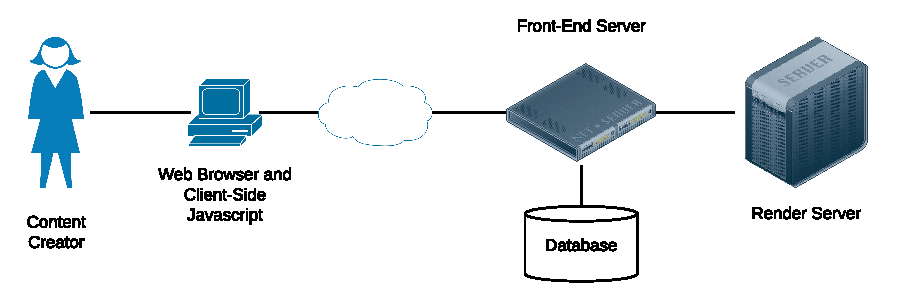
\includegraphics{network-diagram}
  \caption{Network Diagram.}
  \label{fig:network-diagram}
\end{figure}

When a user modifies a video with the tool, the client-side code generates
a computer-readable description of the changes made to the video called an
edit list. The client-side code then sends the edit list to the preview
server. The preview server uses the edit list and the user's original
video (which has already been uploaded to YouTube) to generate a
low-fidelity version of the video. It returns the location of the
low-fidelity preview video to the client-side code, which then displays
the preview video to the user.

The client-side code and front-end server communicate by serializing the
changes made to the video into an edit list, using the JSON format. A
sample edit list is shown in figure~\ref{fig:editlist}.

\begin{figure}
  \centering
  \lstinputlisting{editlist.json}
  \caption{Sample Edit List.}
  \label{fig:editlist}
\end{figure}

\subsection{Positionable/Trimmable Audio}\label{sec:ptaudio}
Positionable/trimmable Audio is a new feature for the AudioSwap tool on
YouTube. It allows the user to position and trim audio tracks on their
video. For example, right before the proposal in a marriage proposal video,
a content creator might choose to overlay the chorus of a romantic song,
trimming the audio so that the proposal can be heard when it is made. The
user interface for positioning and trimming audio is shown in
figure~\ref{fig:overview}.

\begin{figure}
  \centering
  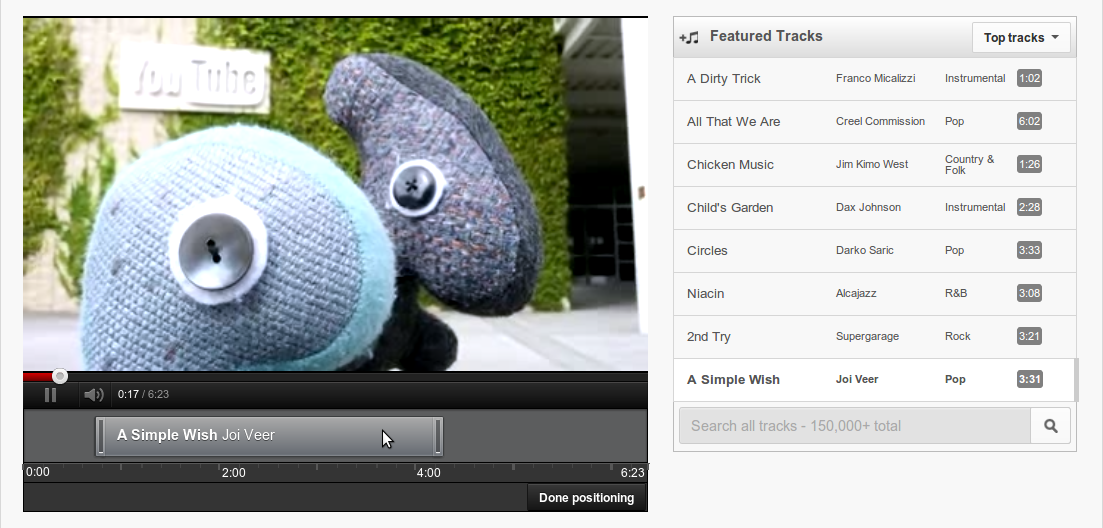
\includegraphics[width=5.515in]{overview}
  \caption{Positionable/Trimmable Audio - User Interface.}
  \label{fig:overview}
\end{figure}

The user can click and drag an audio track, as shown in
figure~\ref{fig:position-drag-start} and
figure~\ref{fig:position-drag-end}. They can also drag the trimming handles
to trim the song, as shown in figure~\ref{fig:trim}.

\begin{figure}
  \centering
  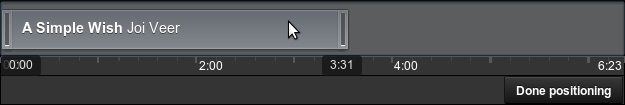
\includegraphics[width=6.25in]{position-drag-start}
  \caption{Positioning Audio (Fig 1 of 2).}
  \label{fig:position-drag-start}
\end{figure}

\begin{figure}
  \centering
  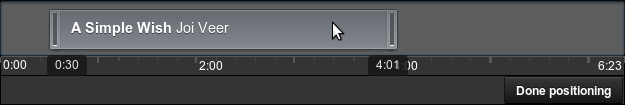
\includegraphics[width=6.25in]{position-drag-end}
  \caption{Positioning Audio (Fig 2 of 2).}
  \label{fig:position-drag-end}
\end{figure}

\begin{figure}
  \centering
  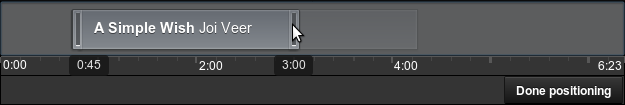
\includegraphics[width=6.25in]{trim}
  \caption{Trimming Audio.}
  \label{fig:trim}
\end{figure}


\subsection{Problem Statement}\label{sec:problem}
When positionable/trimmable audio was first released to content creators,
some content creators noticed a delay between releasing the mouse when
positioning or trimming an audio track and when the preview video would
start playing.

Whenever the user positions or trims an audio track, the edits are
serialized in an edit list and sent to the front-end server. The front-end
server sends a message to tell the render server to render a low-quality
preview of the video, before returning the location of the preview video to
the front-end code. This flow is illustrated in the swimlane activity
diagram in figure~\ref{fig:swimlane}.

\begin{figure}
  \centering
  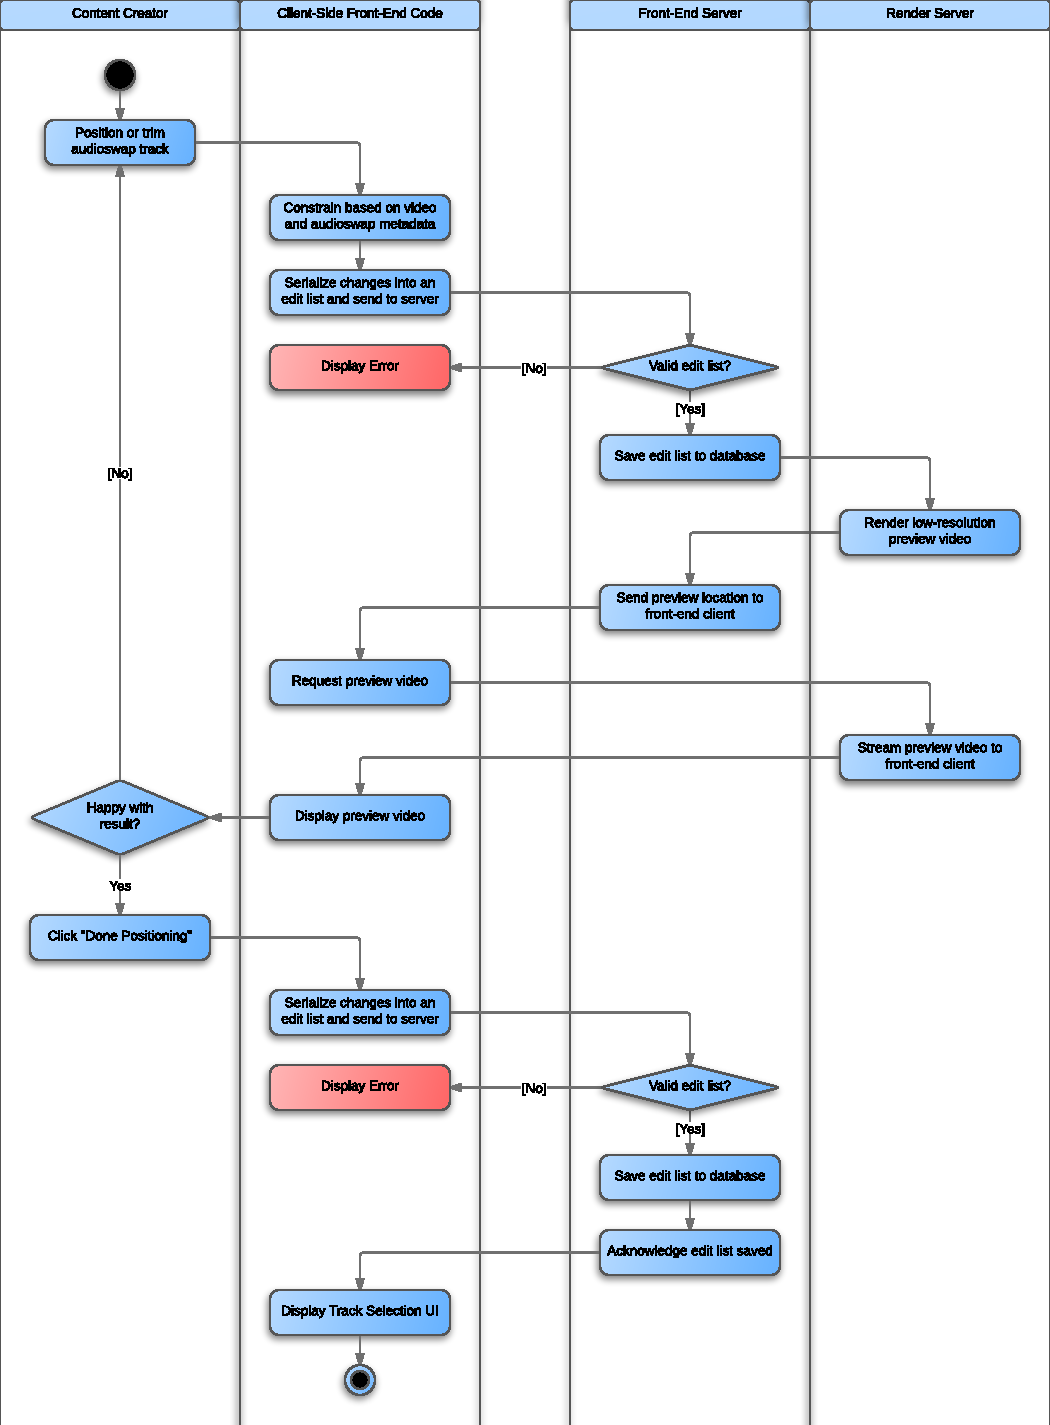
\includegraphics{swimlane}
  \caption{Swimlane Activity Diagram.}
  \label{fig:swimlane}
\end{figure}

A large number of UI events may be generated when the user positions or
trims an audio clip on the video enhancements page. An edit list is generated
for each UI event, with a round-trip to the server and back to process each
event.  This worked fine in development, when each round-trip was virtually
instantaneous. However, this round-trip is estimated to take 600ms for a
typical content creator.\footnote{The calculation to determine this figure is
detailed in appendix~\ref{app:calculating}.}. When a large number of events
occur, the user experiences a large delay before seeing a preview.

This report seeks to select an appropate mitigation strategy for the delay
in the user interface for positionable/trimmable audio.

% You must have either an Analysis or a Synthesis section.
\section{Analysis}
First, a simulation is run to further understand the problem. Then, we
develop criteria and outline various possible mitigation strategies. We use
the weighted sum model,\footnote{This method is covered in MSCI 261, a core
course in the software engineering curriculum at the University of
Waterloo. If you need a refresher, you can read about it on Wikipedia at
\url{http://en.wikipedia.org/wiki/Weighted_sum_model}.} a method of
multi-criteria decision making, to select an alternative. Then, we run
further simulations to tweak the parameters of the chosen alternative.

\subsection{Initial Simulation and Assumptions}\label{sec:assumptions}
In order to protect proprietary design decisions, it is assumed that a
user interaction generates 150 events over five seconds at a constant rate
of 30 events per second. It is also assumed that requests will be
processed one at a time.\footnote{According to \cite{ref:http}, HTTP user
agents should limit themselves to two concurrent requests. It can be seen
in \cite{ref:b423377} that many browsers use more (say, four or six).
However, this is omitted from the simulations for simplicity.}

A simulation of the request queue length for the first 100 seconds after
the start of the interaction is shown in figure~\ref{fig:sim-orig}. Note
that the user does not see the preview until the request queue length drops
to zero, almost 90 seconds after they've stopped adjusting the control.

\begin{figure}
  \centering
  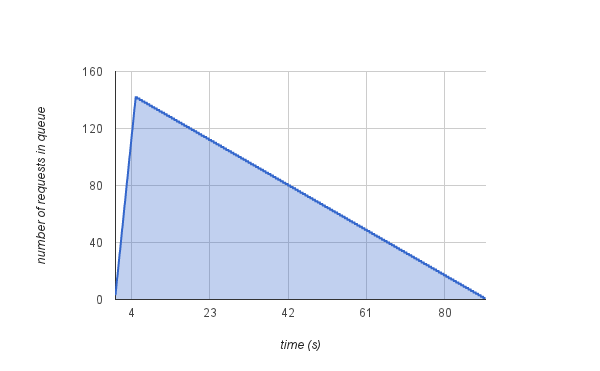
\includegraphics[width=6.25in]{sim-orig}
  \caption{Simulated Request Queue Length (Original Implementation).}
  \label{fig:sim-orig}
\end{figure}

\subsection {Criteria}
Criteria were selected by the team lead, based on past experience and
overall organization priorities.

\subsubsection{Developer Effort}
How much work would a developer need to do to complete this alternative?
(Ranked from 1 (more than one quarter) to 5 (less than one week).)

\subsubsection{PR Impact}
Could we write about the alternative to generate additional interest in the
video enhancement tools? Will pursing an alternative cause others to write
negative articles about the video enhacement tools? (Ranked from 1
(negative impact) to 5 (positive impact).)

\subsubsection{External Dependencies}
Does this alternative depend on deliverables from outside the team? How
likely will those deliverables be ready in a timely manner? (Ranked from
1 (dependencies outside Google) to 5 (no external dependencies).)

\subsubsection{User Impact}
How do we think the user experience will be impacted by this alternative?
(Ranked from 1 (negative impact) to 5 (positive impact).)

\subsubsection{Interest}
Is there someone on the team who is supportive of a particular approach and
willing to do the work to get it done?
(Ranked from 1 (no interest) to 5 (multiple supporters).)

\subsection{Alternatives}
Possible solutions were generated through brainstorming.

\subsubsection{Client-side Audio Syncing}
Synchronize audioswap track and original video playback on the client side,
removing the need for a roundtrip to display the preview for audioswap.

\subsubsection{Do Nothing}
Prioritize other fixes / features instead.

\subsubsection{Real-Time Streaming Preview (WebRTC)}
Replace the video preview player with WebRTC so that we can stream the
preview in real time.

\subsubsection{Throttle Events}
Don't send an edit list to the server for every event. Instead, send one
every $\Delta t$ seconds, as well as one for the "last" event (mouse button up
event).

\subsubsection{Wait for Advances in Networking Technology}
Limit the use of the application to users on super-high-speed network
connections, like Google Fiber.

\subsection{Phase 1: Multi-Criteria Decision Making}
The results of table~\ref{tbl:mcdm} indicate that event throttling is the
best solution. We note that the the solution chosen isn't very robust if
the criteria weights are changed -- in fact, it is possible to make
virtually every solution an "optimal" solution by changing the weights.
However, we proceed with the weights chosen by the team lead, noting that
we should re-evaluate the criteria weights if we need to make a similar
decision in the future.

% Here is a table.  You MUST cite the table in the text before it appears
% in the document.
\begin{table}
  \caption{Multi-Criteria Decision Making Results.}
  \label{tbl:mcdm}
  \centering
  \begin{tabular}{|p{3.0cm}|p{0.75cm}|
                   p{0.75cm}|p{0.75cm}|p{0.75cm}|p{0.75cm}|p{0.75cm}|
                   p{0.75cm}|p{0.75cm}|p{0.75cm}|p{0.75cm}|p{0.75cm}|}
    \hline
    \textbf{Criteria} &
    \textbf{Wt.} &
    \multicolumn{2}{|p{1.50cm}|}{\textbf{Client}} &
    \multicolumn{2}{|p{1.50cm}|}{\textbf{Nothing}} &
    \multicolumn{2}{|p{1.50cm}|}{\textbf{WebRTC}} &
    \multicolumn{2}{|p{1.50cm}|}{\textbf{Throttle}} &
    \multicolumn{2}{|p{1.50cm}|}{\textbf{Wait}} \\
    \hline
    \hline
    Developer Effort &
       2 &  2 &  4 &  5 & 10 &  1 &  2 &  4 &  8 &  5 & 10 \\
    \hline
    PR Impact &
       2 &  3 &  6 &  2 &  4 &  5 & 10 &  3 &  6 &  1 &  2 \\
    \hline
    External Dependencies &
       3 &  2 &  6 &  5 & 15 &  1 &  3 &  5 & 15 &  1 &  3 \\
    \hline
    User Impact &
       2 &  2 &  4 &  3 &  6 &  5 & 10 &  4 &  8 &  1 &  2 \\
    \hline
    Interest &
       1 &  5 &  5 &  1 &  1 &  3 &  3 &  5 &  5 &  1 &  1 \\
    \hline
    \hline
    \textbf{Total} &
      &
      \multicolumn{2}{|r|}{\textbf{25}} &
      \multicolumn{2}{|r|}{\textbf{36}} &
      \multicolumn{2}{|r|}{\textbf{28}} &
      \multicolumn{2}{|r|}{\textbf{42}} &
      \multicolumn{2}{|r|}{\textbf{18}} \\
    \hline
  \end{tabular}
\end{table}

\subsection{Phase 2: Simulation and Optimization}
A number of simulations was performed to determine the best value of
$\Delta t$, the duration between edit lists being sent to the server. A
sample of these simulations is shown below in figure~\ref{fig:sim-300ms},
figure~\ref{fig:sim-600ms}, and figure~\ref{fig:sim-1000ms}. Of the
simulations performed, the value $\Delta t=600 ms$ provided the most
frequent preview updates to the user while maintaining a bounded request
queue size.

\begin{figure}
  \centering
  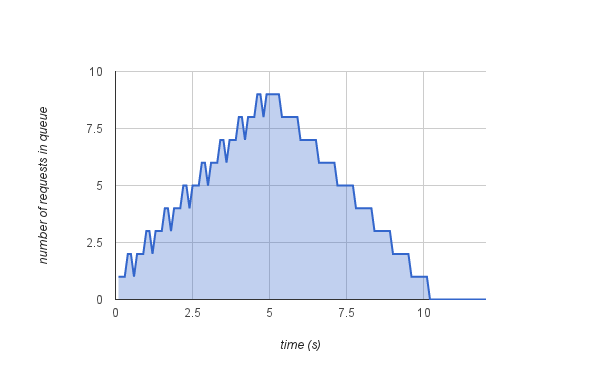
\includegraphics[width=6.25in]{sim-300ms}
  \caption{Simulated Request Queue Length (300ms delay).}
  \label{fig:sim-300ms}
\end{figure}

\begin{figure}
  \centering
  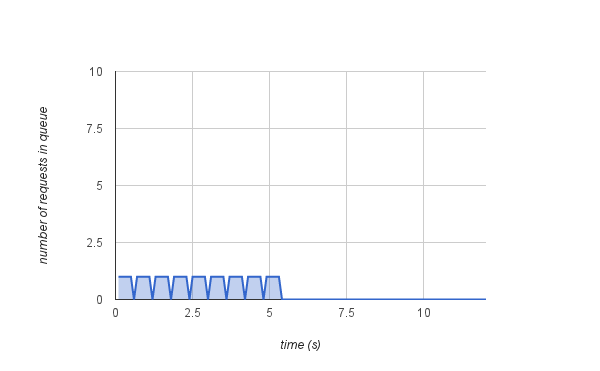
\includegraphics[width=6.25in]{sim-600ms}
  \caption{Simulated Request Queue Length (600ms delay).}
  \label{fig:sim-600ms}
\end{figure}

\begin{figure}
  \centering
  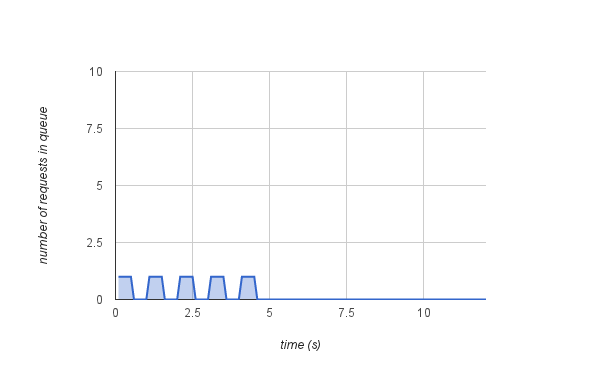
\includegraphics[width=6.25in]{sim-1000ms}
  \caption{Simulated Request Queue Length (1000ms delay).}
  \label{fig:sim-1000ms}
\end{figure}

% You must have a Conclusions section
\section{Conclusions}
The simulation suggests that edit lists should be sent to the front-end
server at most once every 600ms. We note that this value corresponds to the
round-trip time we determined in \S\ref{sec:assumptions}, so we recommend
that an edit list be generated only after the previous one has completed
its round trip,\footnote{With a timeout, of course, and re-transmission
with exponential back-off in the event of packet loss / transient network
failure, etc...} and that UI events only update the UI in the interim.

This provides a bound on the size of the number of requests in the queue.
(Only one request will be processing at any given time.) This, in turn,
gives us a bound on the time between a given user interaction and when the
preview is displayed to the user. (This also reduces the total number of
preview requests sent to the preview server, which results in a
corresponding reduction in CPU and bandwidth usage on the render server.)

% You must have a Recommendations section
\section{Recommendations}
We recommend that the client-side code be modified so that UI events update
the UI immediately, but only trigger a network round-trip if an edit list
is not already in flight.

We note that this recommendation does not necessarily preclude the pursuit
of the other alternatives. Instead, the above alternative should be pursued
first, since it provides the best overall trade-off given the criteria.
Pursuit of the remaining alternative solutions should then be prioritized
within the overall context of the team's objectives and key results (OKRs)
for the quarter.

%%%%%%%%%%%%%%%%%%%%%%%%%%%%%%%%%%%%%%%%%%%%%%%%%%%%%%%%%%%%%%%%%%%%%
%% BACK MATTER
%%%%%%%%%%%%%%%%%%%%%%%%%%%%%%%%%%%%%%%%%%%%%%%%%%%%%%%%%%%%%%%%%%%%%
%% \backmatter will make the \section commands ignore their numbering,
\backmatter

% Here, we insert a References section, which will be formatted properly.
% The list of works you have referenced should be specified in the preamble.
% In this template, the file is uw-wkrpt-bib.bib.
%
% Note, you will need to process the document in a certain order.  First,
% run LaTeX.  The % first pass will allow LaTeX to build a list of 
% references, it may % emit warning messages such as:
%   LaTeX Warning: Reference `app:gnugpl' on page 4 undefined on input line 277.
%   LaTeX Warning: There were undefined references.
% This is normal.  Now you run BiBTeX in order to generate the proper
% layout for the references.  After this, you run LaTeX once more.
\printbibliography[heading=bibintoc]

%%%%%%%%%%%%%%%%%%%%%%%%%%%%%%%%%%%%%%%%%%%%%%%%%%%%%%%%%%%%%%%%%%%%%
%% APPENDICES
%%%%%%%%%%%%%%%%%%%%%%%%%%%%%%%%%%%%%%%%%%%%%%%%%%%%%%%%%%%%%%%%%%%%%
%% \appendix will reset \section numbers and turn them into letters.
%%
%% Don't forget to refer to all your appendices in the main report.
\appendix
\begin{appendices}

\section{Calculating Simulated Server Response Time}\label{app:calculating}
The simulated server response time is comprised by summing multiple
factors, as noted below.

\subsection{Round Trip Time}
Round-trip travel times between three locations in North America and
youtube.com were sampled.

\begin{table}
  \caption{Round Trip Time.}
  \label{tbl:rtt}
  \centering
  \begin{tabular}{|p{2.0cm}|p{2.0cm}|p{2.0cm}|p{2.0cm}|p{2.0cm}|p{2.0cm}|
                   p{2.0cm}|}
    \hline
    \textbf{Location} &
    \textbf{Trial 1} &
    \textbf{Trial 2} &
    \textbf{Trial 3} &
    \textbf{Trial 4} &
    \textbf{Mean} &
    \textbf{Sample StDev} \\
    \hline
    \hline
    Richmond Hill, Ontario &
      7.77 & 7.16 & 6.85 & 7.44 & 7.305 & 0.393 \\
    \hline
    Waterloo, Ontario &
      6.16 & 6.09 & 6.28 & 6.12 & 6.163 & 0.083 \\
    \hline
    Fremont, California &
      1.18 & 1.30 & 1.18 & 1.28 & 1.235 & 0.064 \\
    \hline
    \hline
    \multicolumn{5}{|p{10.0cm}|}{\textbf{Average}} &
      4.901 & 2.759 \\
    \hline
  \end{tabular}
\end{table}

\subsection{Encoding Time}
To protect proprietary design decisions, assume it takes 2000 ms to encode
1000 s (~= 16 minutes) of audio. (Video encoding time is ignored; since
the control only alters the audio track, we assume that existing video
encodes can be reused and multiplexed into the result upon being sent to
the client.) We take the average of the durations of top featured tracks
in the audio enhancement page to get an approximate audio duration of 4
minutes, 53.125 seconds. Based on our assumption, this would take 587 ms
to encode.

\subsection{Wi-Fi}
The use of a wireless network standard such as 802.11n may introduce
additional latency in the HTTP request. The amount of this latency varies
depending on many factors, and could be the subject of its own report. It
is assumed that the user is using a wired connection for the purposes of
this report. It should be noted that the final implementation may need
further adjustment to compensate for the extra latency that users of these
networks will encounter.

\subsection{Other Factors}
It is assumed that other tasks like multiplexing the audio and video
streams on the preview server, and server-side parsing of the edit list
are almost negligible. The duration of these tasks should be dwarfed by
the time taken to encode the audio on the preview server. We add 8 ms of
latency to account for these other factors.

\end{appendices}
\end{document}
